%include part: see main.beamer.tex and main.article.tex
%include common packages and settings
\usepackage{etex} %эта магическая херь избавляет от переполнения регистров TeX а!!!

\mode<article>{\usepackage{fullpage}}
\mode<presentation>{
    \usetheme{Madrid} %%Boadilla,Madrid,AnnArbor,CambridgeUS,Malmoe,Singapore,Berlin
    \useoutertheme{shadow}
} 

\usepackage[utf8]{inputenc}
\usepackage[russian]{babel}
\usepackage{indentfirst}
\usepackage{graphicx}

\usepackage{amsmath}
\usepackage{amsfonts}
\usepackage{amsthm}
\usepackage{algorithm}
\usepackage{algorithmic}

\usepackage[all]{xy}

\date{Лекция по дисциплине <<дискретная математика>>\\(\today)}
\author[М.~М.~Шихов]{Михаил Шихов \\ \texttt{\underline{m.m.shihov@gmail.com}}}

%для рисования графов пакетом xy-pic
\entrymodifiers={++[o][F-]}

%для псевдокода алгоритмов (algorithm,algorithmic)
\renewcommand{\algorithmicrequire}{\textbf{Вход:}}
\renewcommand{\algorithmicensure}{\textbf{Выход:}}
\renewcommand{\algorithmiccomment}[1]{// #1}
\floatname{algorithm}{Псевдокод}



\title[Множества]{Множества}


\begin{document}

%титул и содержание статьи
\mode<article>{\maketitle\tableofcontents}

%титул и содержание презентации
\frame<presentation>{\titlepage}
\begin{frame}<presentation>
    \frametitle{Содержание}
    \tableofcontents
\end{frame}


\section{Базовые понятия теории множеств}

\subsection{Множества}

\begin{frame}
    \frametitle{Множество}
    
    \begin{definition}
        
        \uncover<1>{Множество --- это\ldots}
        
        \uncover<2>{
            Под \alert{множеством} $M$ подразумевается совокупность (набор) некоторых \alert{объектов}, которые будут называться \alert{элементами} множества $M$.
        }
    \end{definition}
    
    \uncover<2>{
        Пусть $M$ --- множество. В отношении объекта $x$ пишут:
        \begin{itemize}
            \item $x\in M$, если $x$ является элементом множества $M$;
            \item $x\not\in M$, если $x$ не является элементом множества $M$;
        \end{itemize}
    }
\end{frame}

\begin{frame}
    \frametitle{Способы задания множеств}
    
    \begin{itemize}
        \item Явным перечислением элементов: $A=\{a,b,c\}$. Кроме того:
            \[
                B=\{1,\{2,3\},\{4,5\}\}.
            \]
        \item Характеристическим предикатом $\{x|P(x)\}$:
            \[
                C=\{x|x\text{ --- четное число}\}.
            \]
        \item Порождающей процедурой: $D=\{x|x=f\}$.
            \begin{algorithm}[H]
                \caption{Функция $f$}
                \begin{algorithmic}[1]
                    \FOR{$i=1$ to $3$}
                        \STATE{$x\gets i^2$}
                        \STATE{\textbf{yeld} $x$} \COMMENT{Возврат значения с продолжением выполнения}
                    \ENDFOR
                \end{algorithmic}
            \end{algorithm}
        
    \end{itemize}
\end{frame}

\begin{frame}
    \frametitle{Cтандартные обозначения множеств}
    
    \begin{itemize}
        \item $\emptyset=\{\}$ --- \alert{пустое} множество.
        \item $\mathbb{U}$ или $1$ --- \alert{универсальное} множество, \alert{универсум}\footnote{От слова universe --- вселенная. Содержит \alert{все} мыслимые объекты}.
        \item $\mathbb{N}=\{0,1,2,\ldots\}$ --- множество натуральных чисел.
        \item $\mathbb{Z}=\{0,\pm 1,\pm 2,\ldots\}$ --- множество целых чисел.
        \item $\mathbb{Q}$ --- множество всех рациональных дробей.
        \item $\mathbb{P}$ --- множество простых чисел.
        \item $\mathbb{R}$ --- множество вещественных (действительных) чисел.
        \item $\mathbb{C}$ --- множество комплексных чисел.
    \end{itemize}
\end{frame}


\subsection{Мощность}

\begin{frame}
    \frametitle{Мощность конечного множества}
    
    \begin{definition}
        Количество элементов в \alert{конечном} множестве $A$ называют \alert{мощностью конечного множества} и обозначают $|A|$.
    \end{definition}
    
    \begin{example}
        \[
            \begin{array}{l}
                |\emptyset|=\uncover<2>{0}\\
                |\{\emptyset\}|=\uncover<2>{1}\\
                |\{1\}|=\uncover<2>{1}\\
                |\{1,2\}|=\uncover<2>{2}\\
                |\{1,\{2,3\}\}|=\uncover<2>{2}
            \end{array}
        \]
    \end{example}
\end{frame}


\subsection{Произведение множеств}

\begin{frame}
    \frametitle{Произведение множеств}
    \framesubtitle{Кортеж}
    
    \begin{definition}
        Упорядоченную последовательность из $n$ элементов $(x_1,x_2,\ldots,x_n)$ будем называть \alert{кортежем} длины $n$. 
    \end{definition}
    
    Элемент $x_i$ называется $i$-й \emph{координатой} кортежа. Два кортежа длины $n$: $(x_1,x_2,\ldots,x_n)$ и $(y_1,y_2,\ldots,y_n)$ равны тогда и только тогда, когда $x_1=y_1$, $x_2=y_2$, \ldots, $x_n=y_n$.
    
    \begin{example}
        \[(1,2)\neq(2,1)\]
        \[(1,(2,3))=(1,(2,3))\]
    \end{example}
\end{frame}

\begin{frame}
    \frametitle{Декартово произведение множеств}

    \begin{definition}
        \alert{Декартовым} (прямым) произведенем множеств $A_1,A_2,\ldots,A_n$ называется множество 
        \[\{(x_1,x_2,\ldots,x_n)|x_1\in A_1,x_2\in A_2,\ldots,x_n\in A_n\},\]
        обозначаемое через $A_1\times A_2\times\cdots\times A_n$ или $\displaystyle\prod_{i=1}^{n}A_i$.
    \end{definition}

    Видно, что $A\times B\neq B\times A$. 
    \begin{example}[Произведение $A=\{a,b\}$ и $B=\{1,2\}$]
        \begin{itemize}
            \item $A\times B=$\uncover<2>{$\{(a,1),(b,1),(a,2),(b,2)\}$;}
            \item $B\times A=$\uncover<2>{$\{(1,a),(1,b),(2,a),(2,b)\}$;}
        \end{itemize}
    \end{example}
\end{frame}

\begin{frame}
    \frametitle{Степень множества}
    
    \begin{definition}
        Если $A_1=A_2=\ldots=A_n=A$, то множество $A_1\times A_2\times\cdots\times A_n$ называется $n$-й \alert{степенью} множества $A$ и обозначается как $A^n$. 
    \end{definition}
    
    По определению: $A^0=\{\emptyset\}$.
    \begin{example}[Степени $A=\{a,b\}$]
        \begin{itemize}
            \item $A^0=\{\emptyset\}$.
            \item $A^1=A=\{a,b\}$.
            \item $A^2=\{(a,a),(a,b),(b,a),(b,b)\}$.
            \item             
                \(A^3=\left\{
                    \begin{array}{c}
                        (a,a,a),(a,a,b),(a,b,a),(a,b,b),\\
                        (b,a,a),(b,a,b),(b,b,a),(b,b,b)
                    \end{array}
                    \right\}.
                \)
        \end{itemize}
    \end{example}    
\end{frame}


\section{Отношения между множествами}


\subsection{Виды отношений}

\begin{frame}
    \frametitle{Отношения между множествами}
    \framesubtitle{Отношение нестрогого включения $\subseteq$}
    
    \begin{definition}
        Множество $A$ \alert{содержится} в множестве $B$ (множество $B$ \alert{включает} множество $A$), если каждый элемент $A$ есть элемент $B$
    \end{definition}
    
    \[A\subseteq B, \text{ если } (x\in A)\Rightarrow (x\in B).\]
    В этом случае:
    \begin{itemize}
        \item $A$ --- \alert{подмножество};
        \item $B$ --- \alert{надмножество};
    \end{itemize}
    
    Запись $B\supseteq A$ эквивалентна $A\subseteq B$. Справедливо также:
    \begin{itemize}
        \item $M\subseteq M$;
        \item $\emptyset\subseteq M$.
    \end{itemize}
\end{frame}

\begin{frame}
    \frametitle{Отношения между множествами}
    \framesubtitle{Отношение строгого включения $\subset$}
    
    \begin{definition}
        Множество $A$ называется \alert{собственным} подмножеством множества $B$, если $A$ является подмножеством множества $B$, и если $B$ не является подмножеством $A$
    \end{definition}
    
    \[A\subset B,\text{если $(A\subseteq B)\land(B\not\subseteq A)$}\]
    
    Запись $B\supset A$ эквивалентна $A\subset B$.
\end{frame}

\begin{frame}
    \frametitle{Отношения между множествами}
    \framesubtitle{Равенство множеств}
    
    \begin{definition}
        Множества $A$ и $B$ \alert{равны} (обозначается $A=B$), если $A$ подмножество $B$ и $B$ подмножество $A$
    \end{definition}
    
    \[(A=B)\Leftrightarrow(A\subseteq B\land B\subseteq A)\]
    
    \begin{example}[Равны ли множества?]
        \[
            \begin{array}{c}
                \{1,2,3\}\uncover<2>{=}\{2,1,3\}\\
                \{1,\{a,b\},2\}\uncover<2>{=}\{\{b,a\},2,1\}\\
                \{1,(a,b),2\}\uncover<2>{\neq}\{(b,a),2,1\}
            \end{array}
        \]
    \end{example}
\end{frame}

\begin{frame}
    \frametitle{Отношения между множествами}
    \framesubtitle{Общее положение множеств}
    
    \begin{definition}
        Множества $A$ и $B$ находятся в \alert{общем положении} (обозначается $\text{ОП}(A,B)$), если одновременно выполняются три условия:
        
        \begin{enumerate}
            \item $\exists x (x\in A \land  x\not\in B)$,
            \item $\exists y (y\in B \land  y\not\in A)$,
            \item $\exists z (z\in A \land  z\in B)$.
        \end{enumerate}
    \end{definition}
\end{frame}

\begin{frame}
    \frametitle{Отношения между множествами}
    \framesubtitle{Не имеющие общих элементов}
    
    \begin{definition}
        Множества $A$ и $B$ \alert{не имеют общих элементов} (обозначается $A\cap B=\emptyset$), если выполняется:
        \[
            (A\not\subseteq B)\land(B\not\subseteq A)
        \]
    \end{definition}
\end{frame}

\begin{frame}
    \frametitle{Отношения между множествами}
    \framesubtitle{Два множества $A$ и $B$ могут находиться лишь в одном из следующих отношений}
    
    \begin{enumerate}
        \item $A=B$;
        \item $A\subset B$;
        \item $A\supset B$;
        \item $\text{ОП}(A,B)$;
        \item $A\cap B = \emptyset$.
    \end{enumerate}
    
    \begin{center}
        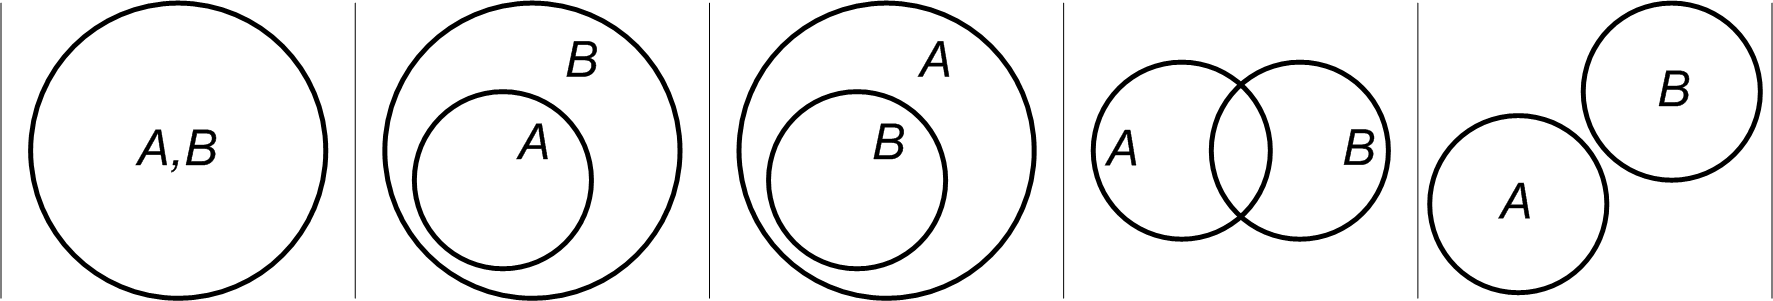
\includegraphics[width=\textwidth]{fig/setRelations}
    \end{center}
\end{frame}


\subsection{Булеан}

\begin{frame}
    \frametitle{Булеан}

    \begin{definition}
        Множество всех подмножеств множества $M$ называется \alert{булеаном} и обозначается $2^M$:
        
        \[2^M=\{A|A\subseteq M\}\]
    \end{definition}

    \uncover<1>{Сколько элементов в булеане конечного множества $M$?}
    
    \uncover<2->{Для конечного множества $M$ справедливо $\left|2^M\right|=2^{\left|M\right|}$}
    
    \uncover<3->{
        \begin{example}[Булеан множества $M=\{a,b,c\}$]
            $2^M=$\uncover<4>{$\{\emptyset, \{a\}, \{b\}, \{c\}, \{a,b\}, \{a,c\}, \{b,c\}, \{a,b,c\}\}$}
        \end{example}        
    }
\end{frame}


\section{Алгебра множеств}


\subsection{Операции над множествами}

\begin{frame}
    \frametitle{Алгебра множеств}
    \framesubtitle{Основные операции алгебры множеств}
    
    \begin{enumerate}
        \item Объединение:\[A\cup B=\{x|x\in A \lor x\in B\}.\]
        
        \item Пересечение:\[A\cap B=\{x|x\in A \land x\in B\}.\]
        
        \item Дополнение:\[\overline{A}=\{x|x\not\in A\}.\]
    \end{enumerate}
\end{frame}

\begin{frame}
    \frametitle{Алгебра множеств}
    \framesubtitle{Основные операции алгебры множеств}
    
    \begin{center}
        \begin{tabular}{ccc}
            \includegraphics[width=.3\textwidth]{fig/ABSetOr}
                & \includegraphics[width=.3\textwidth]{fig/ABSetAnd}
                    & 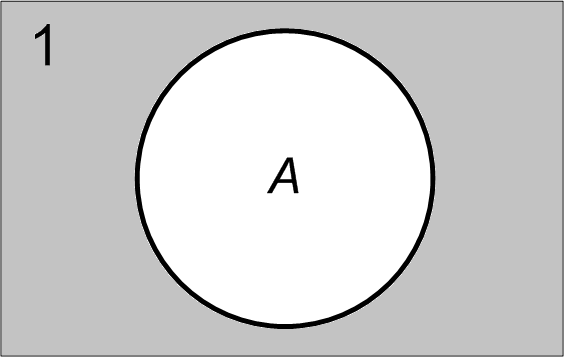
\includegraphics[width=.3\textwidth]{fig/ASetNot}
                        \\
            $A\cup B$ 
                & $A\cap B$
                    & $\overline{A}$
        \end{tabular}
    \end{center}
    
    \begin{itemize}
        \item $\{1,3,2\}\cup\{0,2,4,3\}=\uncover<2>{\{0,1,2,3,4\}}$
        \item $\{1,3,2\}\cap\{0,2,4,3\}=\uncover<2>{\{2,3\}}$
        \item При $\mathbb{U}=\{0,1,2,3\}$: $\overline{\{2,1\}}=\uncover<2>{\{0,3\}}$
    \end{itemize}
\end{frame}

\begin{frame}
    \frametitle{Алгебра множеств}
    \framesubtitle{Дополнительные операции алгебры множеств}
    
    \begin{enumerate}
        \item Разность:
        \[
            A\backslash B=A\cap\overline{B}=\{x|x\in A \land x\not\in B\}.
        \]
        
        \item Симметрическая разность:
        \[
            \begin{split}
                A\Delta B=(A\backslash B)\cup(B\backslash A)=(A\cup B)\backslash(A\cap B)=\\
                =\{x|(x\in A \land x\not\in B)\lor(x\not\in A\land x\in B)\}.
            \end{split}
        \]
    \end{enumerate}
\end{frame}

\begin{frame}
    \frametitle{Алгебра множеств}
    \framesubtitle{Дополнительные операции алгебры множеств}
    
    \begin{center}
        \begin{tabular}{cc}
            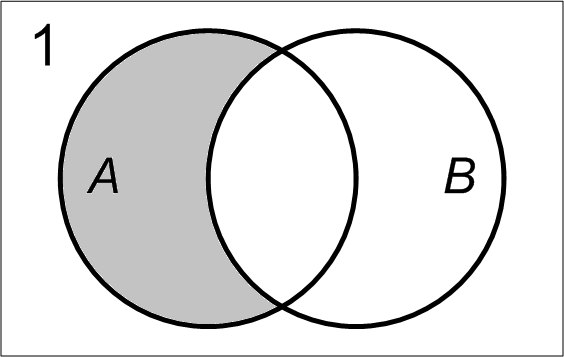
\includegraphics[width=.3\textwidth]{fig/ABSetSub}
                & 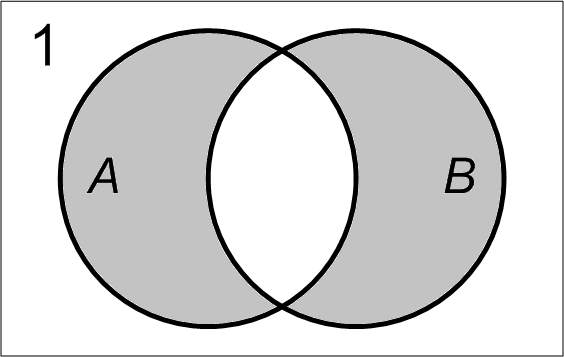
\includegraphics[width=.3\textwidth]{fig/ABSetSymSub}
                    \\
            $A\backslash B$ 
                & $A\Delta B$
        \end{tabular}
    \end{center}
    
    \begin{itemize}
        \item $\{1,3,2\}\backslash\{0,2,4,3\}=\uncover<2>{\{1\}}$
        \item $\{1,3,2\}\Delta\{0,2,4,3\}=\uncover<2>{\{0,1,4\}}$
    \end{itemize}    
\end{frame}

\begin{frame}
    \frametitle{Алгебра множеств}
    \framesubtitle{Общее положение множеств}
    
    \begin{center}
        \begin{tabular}{cc}
            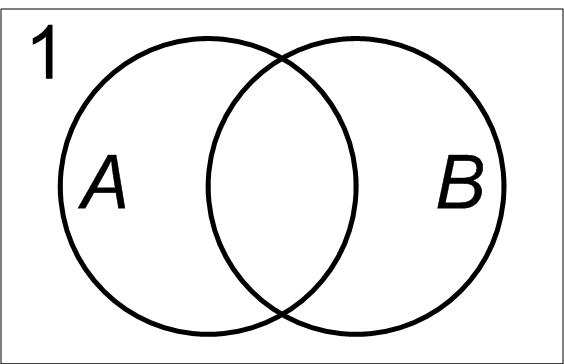
\includegraphics[width=.3\textwidth]{fig/ABcommon}
                & 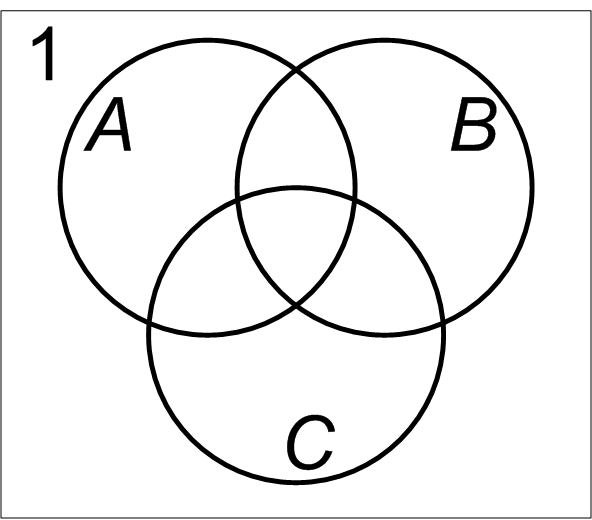
\includegraphics[width=.3\textwidth]{fig/ABCcommon}
                    \\
            \begin{tabular}{l}
                $A=\uncover<2->{\{1,3\}}$\\
                $B=\uncover<2->{\{3,2\}}$
            \end{tabular}
                & 
                \begin{tabular}{l}
                    $A=\uncover<3>{\{4,5,6,7\}}$\\
                    $B=\uncover<3>{\{2,3,6,7\}}$\\
                    $C=\uncover<3>{\{1,3,5,7\}}$
                \end{tabular}
        \end{tabular}
    \end{center}
    
\end{frame}

\begin{frame}
    \frametitle{Алгебра множеств}
    \framesubtitle{Аналитическое задание множеств}
    
    \begin{center}
        \begin{tabular}{ccc}
            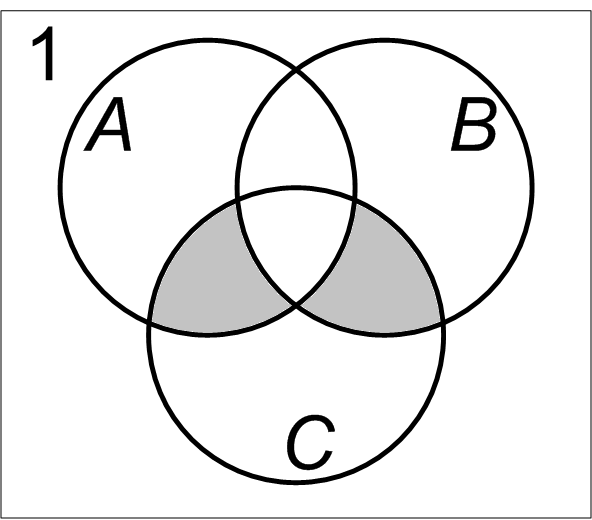
\includegraphics[width=.3\textwidth]{fig/ABCsposa}
                & 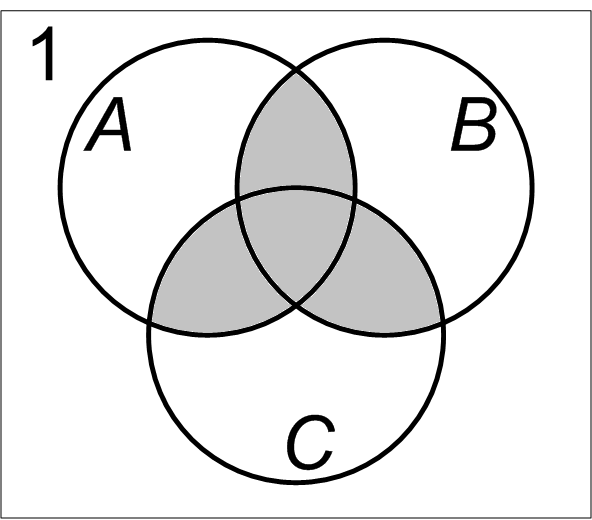
\includegraphics[width=.3\textwidth]{fig/ABCsposb}
                    & 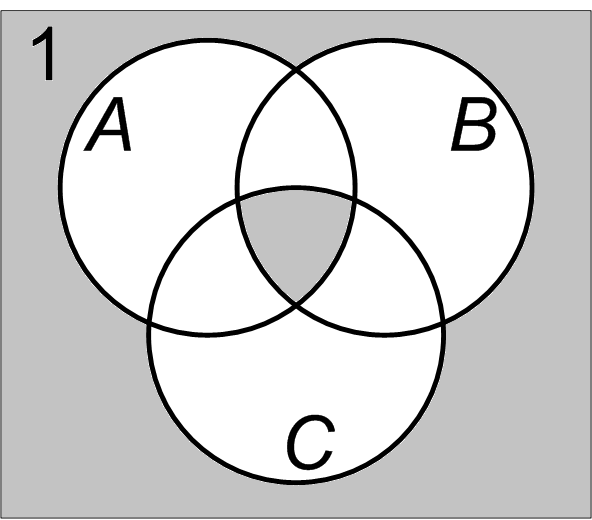
\includegraphics[width=.3\textwidth]{fig/ABCsposc}
                        \\
            \(\uncover<2->{
                \begin{array}{r}
                    ((A\cup B)\cap C)\cap\\
                    \cap\overline{A\cap B}
                \end{array}
            }\)
                & 
                \(\uncover<3->{
                    \begin{array}{r}
                        (A\cap B)\cup(A\cap C)\cup\\
                        \cup(B\cap C)
                    \end{array}
                }\)
                    & 
                    \(\uncover<4>{
                        \begin{array}{r}
                            (\overline{A\cup B\cup C})\cup\\
                            \cup(A\cap B\cap C)
                        \end{array}
                    }\)
        \end{tabular}
    \end{center}
    
\end{frame}

\begin{frame}
    \frametitle{Алгебра множеств}
    \framesubtitle{Аналитическое задание множеств}
    
    Множества $A$, $B$, $C$ в общем положении. 
    
    Диаграммой Эйлера-Венна изобразить множество:
    \begin{enumerate}
        \item $\overline{A}\cap\overline{B}$
        \item $\overline{A}\cup\overline{B}$
        \item $(A\cup B)\cap(\overline{C\cup (A\cap B)})$
        \item $((A\cup B)\cap\overline{C})\cup(A\cap B)$
    \end{enumerate}
\end{frame}

\begin{frame}[allowframebreaks]
    \frametitle{Алгебра множеств}
    \framesubtitle{Свойства операций}
    
    \begin{enumerate}
        \item идемпотентность:
        \[A\cup A=A, A\cap A=A;\]
        
        \item коммутативность:
        \[A\cup B=B\cup A, A\cap B=B\cap A;\]
        
        \item ассоциативность:
        \[(A\cup B)\cup C=A\cup(B\cup C), (A\cap B)\cap C=A\cap(B\cap C);\]
        
        \item дистрибутивность:
        \[A\cup(B\cap C)=(A\cup B)\cap(A\cup C),A\cap(B\cup C)=(A\cap B)\cup(A\cap C);\]
        
        \item законы де М\'{о}ргана:
        \[
            \overline{A\cap B}=\overline{A}\cup\overline{B},
            \overline{A\cup B}=\overline{A}\cap\overline{B};
        \]
        
        \item поглощение:
        \[(A\cup B)\cap A=A,(A\cap B)\cup A=A;\]
        
        \item свойства нуля (пустого множества $\emptyset$):
        \[(A\cup \emptyset)=A,(A\cap \emptyset)=\emptyset;\]
        
        \item свойства единицы (универсального множества $1$):
        \[(A\cup 1)=1,(A\cap 1)=A;\]
        
        \item инволютивность:
        \[\overline{\overline{A}}=A;\]
            
        \item свойства дополнения:
        \[
            \overline{A}\cup A=1,
            \overline{A}\cap A=\emptyset;
        \]
        
        \item выражение разности:
        \[
            A\backslash B=A\cap\overline{B}.
        \]
    \end{enumerate}
\end{frame}

\begin{frame}
    \frametitle{Алгебра множеств}
    \framesubtitle{Доказательства утверждений алгебры множеств}
    
    \begin{example} 
        Докажем закон де М\'{о}ргана для случая $\overline{A\cup B}=\overline{A}\cap\overline{B}$. 
    \end{example}
    \begin{proof}
        Докажем, что $\overline{A\cup B}\subseteq\overline{A}\cap\overline{B}$ и $\overline{A}\cap\overline{B}\subseteq\overline{A\cup B}$.
        \begin{enumerate}
            \item $\overline{A\cup B}\subseteq\overline{A}\cap\overline{B}$. Возьмем $x\in \overline{A\cup B}$. Тогда $x\not\in A\cup B$. Следовательно $x\not\in A$ и $x\not\in B$. То есть $x\in\overline{A}$ и $x\in\overline{B}$. Тогда по определению $x\in\overline{A}\cap\overline{B}$.
            \item $\overline{A}\cap\overline{B}\subseteq\overline{A\cup B}$. Возьмем $x\in\overline{A}\cap\overline{B}$. Тогда $x\in\overline{A}$, а значит $x\not\in A$. Аналогично делаем вывод, что $x\not\in B$. Стало быть $x\not\in(A\cup B)$, а значит $x\in\overline{A\cup B}$.
        \end{enumerate}
    \end{proof}
\end{frame}

\begin{frame}
    \frametitle{Алгебра множеств}
    \framesubtitle{Базис. Избыточность основных операций}
    
    \begin{itemize}
        \item $\overline{A}$
        \item $A\cap B$
        \item<1> $A\cup B$
    \end{itemize}
    
    \uncover<2>{
        \[A\cup B=\overline{\overline{A}\cap\overline{B}}\]
    }
\end{frame}

\begin{frame}
    \frametitle{Алгебра множеств}
    \framesubtitle{Базис одной операции}
    
    Одной операцией вычитания можно заменить:
    \begin{itemize}
        \item $\overline{A}=\uncover<2>{1\backslash A;}$
        \item $A\cap B=\uncover<2>{A\backslash (1\backslash B).}$
    \end{itemize}
\end{frame}


\subsection{Преобразования множеств}

\begin{frame}
    \frametitle{Алгебра множеств}
    \framesubtitle{Аналитические преобразования множеств}
    
    \begin{example}[Аналитические преобразования множеств]
        \[
            \begin{split}
            A\backslash ((A\cup B)\backslash B) = A\cap\overline{((A\cup B)\cap\overline{B})}=\\
            =A\cap(\overline{(A\cup B)}\cup\overline{\overline{B}})=A\cap((\overline{A}\cap\overline{B})\cup B)=\\
            =A\cap((\overline{A}\cup B)\cap\underbrace{(\overline{B}\cup B)}_1)=A\cap (\overline{A}\cup B) = \underbrace{(A\cap\overline{A})}_\emptyset\cup(A\cap B)=\\
            =A\cap B
        \end{split}
        \]
    \end{example}
\end{frame}

\begin{frame}
    \frametitle{Алгебра множеств}
    \framesubtitle{Аналитические преобразования множеств}
    
    \begin{example}[Аналитические преобразования множеств]
        \[
            \begin{split}
                \overline{((C\backslash A)\backslash B)}\cap A=
                \uncover<2>{
                    \overline{((C\backslash A)\cap\overline{B})}\cap A=
                    (\overline{(C\backslash A)}\cup\overline{\overline{B}})\cap A=\\
                    =(\overline{(C\backslash A)}\cup B)\cap A=
                    (\overline{(C\cap\overline{A})}\cup B)\cap A=
                    ((\overline{C}\cup\overline{\overline{A}})\cup B)\cap A=\\
                    =((\overline{C}\cup A)\cup B)\cap A=
                    ((A\cup\overline{C})\cup B)\cap A=
                    (A\cup(\overline{C}\cup B))\cap A=\\=A
                }
            \end{split}
        \]
    \end{example}
\end{frame}


\subsection{Семейства подмножеств множества}

\begin{frame}
    \frametitle{Алгебра множеств}
    \framesubtitle{Семейства, покрытия и разбиения}

    $\mathcal{E}=\{E_i|i\in\mathbb{N}\land E_i\subset M\}$ называется \alert{семейством} подмножеств множества $M$. Cемейство $\mathcal{E}$ называют \alert{покрытием} множества $M$, если каждый элемент $M$ содержится хотя бы в одном $E_i$:
    \[
        M\subseteq\bigcup_{i\in\mathbb{N}}E_i
        \Leftrightarrow
        \forall x\in M~\exists i\in\mathbb{N}~x\in E_i
    \]
    Семейство $\mathcal{R}$ называют \alert{разбиением}, если множества $E_i$ попарно не пересекаются:
    \[
        \forall i,j\in\mathbb{N}~i\neq j\Rightarrow E_i\cap E_j=\emptyset
    \]
    \begin{example}[Чем являются семейства подмножеств $M$: $\mathcal{E}_1$, $\mathcal{E}_2$?]
        $M=\{0,1,2,3,4\}$, 
        $\mathcal{E}_1=\{\{4,1\},\{2\},\{3,0\}\}$,
        $\mathcal{E}_2=\{\{2,1,3\},\{0,4,2\}\}$.
    \end{example}
\end{frame}


\appendix

%TODO представление множеств в компьютере
\begin{frame}
    \frametitle{Представление множеств в компьютере}
    
    \begin{center}
        ?
    \end{center}
\end{frame}


\begin{frame}
    \frametitle{В заключение}
    
    Множество --- фундаментальное понятие всей дискретной математики. Для углубленного изучения рекомендуются \cite{bib:sudoplatov:discrmath, bib:haggard:discrmathprogrammer, bib:novic:discrmathprogrammer}.
\end{frame}


\begin{frame}[allowframebreaks]{Библиография}
    \bibliographystyle{gost780u}
    \bibliography{./../../bibliobase}
\end{frame}

\end{document}